\documentclass[parskip=full]{scrartcl}
\usepackage[utf8]{inputenc} % use utf8 file encoding for TeX sources
\usepackage[T1]{fontenc}    % avoid garbled Unicode text in pdf
\usepackage[english]{babel}  % english hyphenation, quotes, etc
\usepackage[colorlinks=true,linkcolor=blue]{hyperref}       % detailed hyperlink/pdf configuration
\usepackage{graphicx}       % provides commands for including figures
\usepackage{csquotes}       % provides \enquote{} macro for "quotes"
\usepackage{enumitem}
\usepackage{multicol}
\setlength{\columnsep}{4cm}
%\usepackage{lscape}	% provides landscape portrait

\usepackage{pdflscape}	% provides horizental landscape portrait


\usepackage{pdfpages}	% add another pdf in  Latex

\usepackage{tikz}


\usepackage{verbatim}	% provides multi-line comments

\usepackage{afterpage}
\usepackage{ragged2e}
\usepackage[export]{adjustbox}
\newcommand\tab[1][1cm]{\hspace*{#1}}


\title{\Huge \textbf{HePICS Implementation Document}}
\date{\today \vspace{+10ex}}
\author{Andres Stober \\
	\and Mehyar Cherni \\
	\and Ibrahim Bouriga \\ 
	\and Linjuan Fan \\
	\and Bahaa Mahjane \\ }

\begin{document}

\maketitle
\thispagestyle{empty}

\begin{tikzpicture}[remember picture, overlay]
  \node [anchor=north west, inner sep=0.5pt, yshift=-20pt,xshift=20pt]  at (current page.north west)
     {
\includegraphics[height=1.9cm]{Logo_KIT}};
\end{tikzpicture}

\begin{figure}[b]
\centering
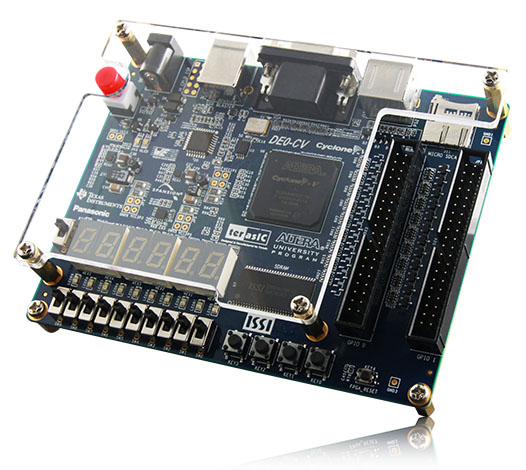
\includegraphics[width=0.45\textwidth, center]{boardimage}
\end{figure}

\pagebreak

\tableofcontents
\thispagestyle{empty}
\pagebreak



\section {Introduction}
	\tab In this document you will find a full description of the work flow in the implementation phase as well as the deviations and changes made on the class digaram. Those changes are sometimes necessary and have convincing reasons that will be mentioned in details.
	\subsection{Workflow}
	\tab In order to distribute tasks and maintain good communication between team members, we use a scrum framework online 	\url{https://app.vivifyscrum.com} and a github repository \url{https://github.com/Turon42/hepics}.
	
	\subsection{Tasks}
	\tab The project can be devided in six parts:
	\tab \begin{itemize}
	\item GUI \ref{GUI}
	\item Image and Neural Network Model  \ref{Image and Neural Network Model}
	\item Sheduler \ref{Scheduler}
	\item Connecting PFGA \ref{Connecting FPGA}
	\item Operation Modes  \ref{Operation Modes}
	\end{itemize}
	
\section{GUI} \label{GUI}
	@Linjuan Fan \textit{(No description provided yet)}
	\begin{center}
		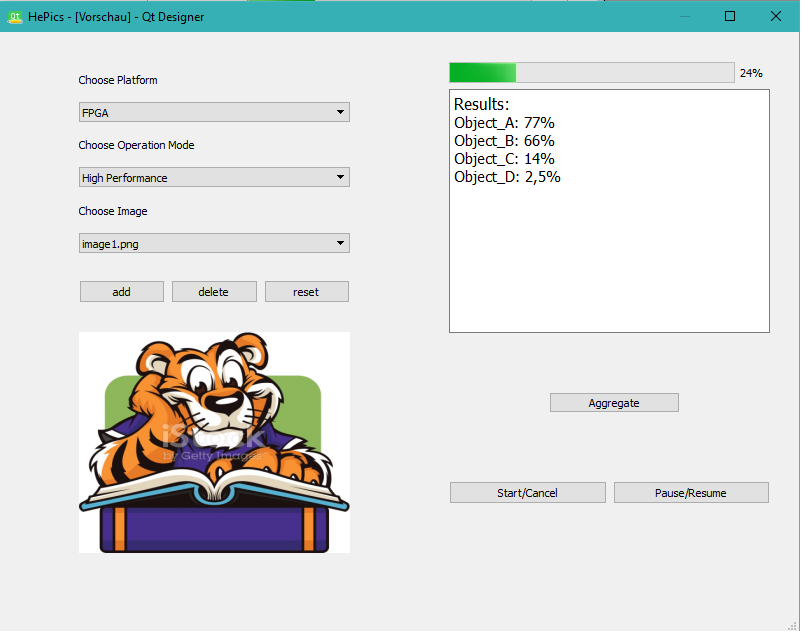
\includegraphics[width=0.9\textwidth]{NewMainWindow}
	\end{center}


\pagebreak

\section {Image and Neural Network Model} \label{Image and Neural Network Model}
	@Ibrahim Bouriga
	
	\subsection {Image Model}
	\tab The Image Class represents the \textbf{input} as well as the \textbf{filter} used in the different layers.\\
	The Image Manger Class however was removed in the implementation because all of its methods can be fully implemented as static ones in the Image Class.\\ As a result the use of this methods does not require any new instance object to be created and thus makes less use of memory.\\ Here a list of of static methods implemented in Image:
	\begin {itemize}
		\item load\_image\_color: load an image
		\item load\_image: load an image an resize it if necessary
		\item load\_image\_stb: uses an external library to load an image. See \ref{External Libraries}
	\end{itemize}

	\subsection {Network Model}
	\tab The Network Model consists of the network and the layers:
	
		\subsubsection {Network}
		\tab The Network Class was implemented as it was introduced in the class diagram. However displaying the topology was not part of the implementation due to the fact that only the alexnet architecture will be deployed in the classification process.
		The architecure (See \ref{fig:alexnet-architecture}) itself was described in a comprehensible configuration file, which will be parsed (See Parser \ref{Parser}) to extract relevant informations about the network.
		
		\subsubsection {Layer}
		\tab The Layer Class stores informations such as the number of inputs and outputs as well as the layer type and define the forward function which is implemented by derived classes:\\
		\begin{itemize}
			\item Convolutional Layer
			\item Max Pool Layer
			\item Connected Layer
			\item Softmax Layer
		\end{itemize}
		\begin{figure}
			\centering
			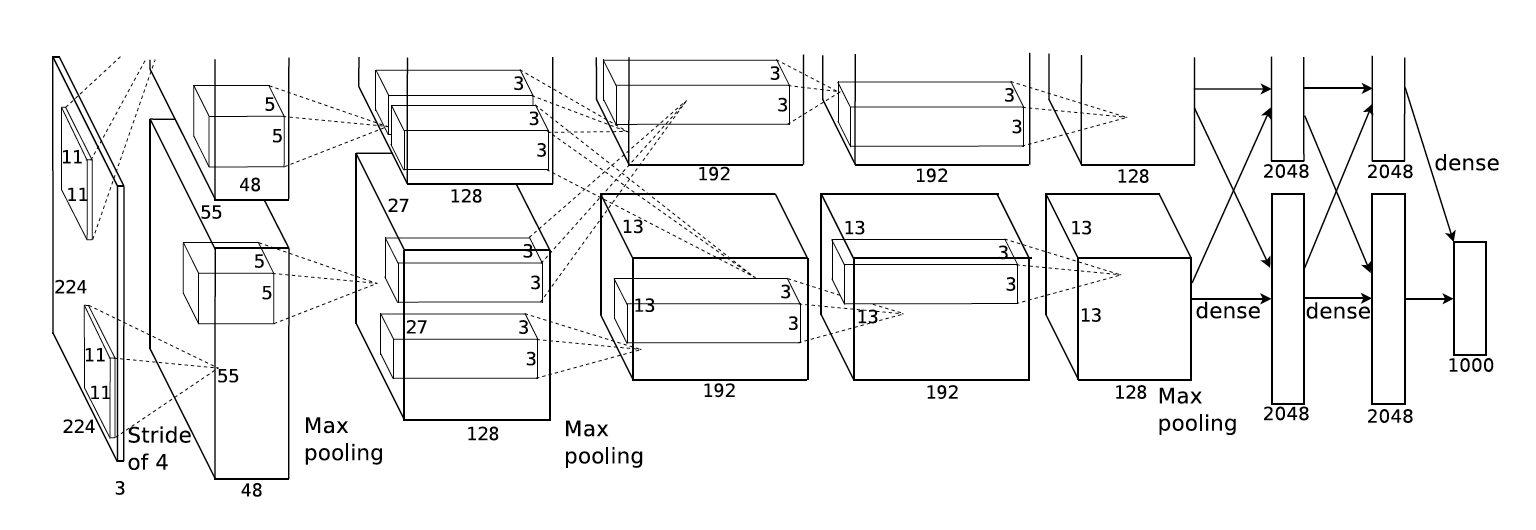
\includegraphics[width=1.0\textwidth]{alexnet-architecture}
			\caption{alexnet architecture}
			\label{fig:alexnet-architecture}
		\end{figure}
		
		\subsubsection {Activation}
		\tab The Activation Class implements the following activations functions:
		\begin{itemize}
			\item ReLu $g(z) = max{0, z}$
			\item Linear $g(z) =z$
			\item Tanh  $g(z) = (e^z -e^{-z}) / (e^z + e^{-z})$
			\item Sigmoid $g(z) = 1 / (1 + e^{-z})$
		\end{itemize}
		
	\subsection {New Classes}
		\paragraph{a.Parser} \label{Parser}
		\tab This class was created to parse and extract informations related to the network from the alexnet architecture (See \ref{fig:alexnet_architecture}).
		\begin{itemize}
			\item parse\_convolutional: create a convolutional layer from the convolution section in the configuration file
			\item parse\_maxpool: create a maxpool layer from the convolution section in the configuration file
			\item parse\_connected: create a connected layer from the convolution section in the configuration file
			\item parse\_softmax: create a softmax layer from the convolution section in the configuration file
			\item load\_network: create the network and initialize layers
		\end{itemize}
		
		\paragraph{b.Utils}
		\tab This class implements static methods that does logically not belong to any object. For instance file and memory errors. 
		
		\paragraph{c.Options\_list}
		\tab This class read datas from the configuration file line by line.\\
		It models a hash set with key words and associated values. The extracted values will be stored in lists (See \ref{Structures})
		
	\subsection {External Libraries} \label{External Libraries}
		\begin{itemize}
			\item stb\_image
			\item GEMM
			\item BLAS
			\item IM2COL
		\end{itemize}
		
	\subsection{Structures} \label{Structures}
		\tab Some availabe structures were implemented again in order to avoid unexpected behaviour like:
		\begin{itemize}
			\item List
			\item Node
		\end{itemize} 
		
\pagebreak

\section{Scheduler} \label{Scheduler}
	@Mehyar Cherni \textit{(No description provided yet)}
	
	
\pagebreak

\section{Connecting FPGA} \label{Connecting FPGA}
	@Andres Stober \textit{(No description provided yet)}
	

\pagebreak



\pagebreak

\section{Operation Modes} \label{Operation Modes}
	\textit{(No description provided yet)}


\pagebreak


\end{document}